\documentclass[dvisvgm,tikz,border=4pt]{standalone}
\usepackage{amsmath,amssymb}

\usetikzlibrary{arrows.meta,positioning,automata,shapes,shapes.misc,calc,decorations.pathmorphing,decorations.markings,angles,quotes,patterns,mindmap,matrix,knots,hobby,trees}
\tikzset{->-/.style={decoration={markings, mark=at position 0.5 with {\arrow{Stealth}}}, postaction={decorate}}}
\begin{document}
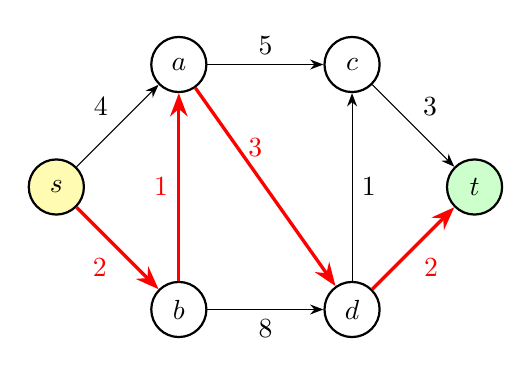
\begin{tikzpicture}[>=Stealth, node distance=2.2cm, v/.style={circle, draw, thick, minimum size=7mm}]
\node[v, fill=yellow!30] (s) {$s$};
\node[v] (a) [above right of=s] {$a$};
\node[v] (b) [below right of=s] {$b$};
\node[v] (c) [right of=a] {$c$};
\node[v] (d) [right of=b] {$d$};
\node[v, fill=green!20] (t) [below right of=c] {$t$};
\draw[->] (s) -- node[above left] {4} (a);
\draw[->, very thick, red] (s) -- node[below left] {2} (b);
\draw[->] (a) -- node[above] {5} (c);
\draw[->, very thick, red] (b) -- node[left] {1} (a);
\draw[->] (b) -- node[below] {8} (d);
\draw[->, very thick, red] (a) -- node[right, pos=0.3] {3} (d);
\draw[->] (c) -- node[above right] {3} (t);
\draw[->, very thick, red] (d) -- node[below right] {2} (t);
\draw[->] (d) -- node[right] {1} (c);
\end{tikzpicture}
\end{document}
